\documentclass[a4paper,11pt]{article}
\usepackage{graphicx} % Required for inserting images
\usepackage[utf8]{inputenc}
\usepackage{float}
\usepackage{pdfpages}
% stops indents on new lines
\setlength\parindent{0pt}
\setlength{\parskip}{0.5em} % afstand efter afsnit

\usepackage{newclude}

\usepackage[
backend=biber,
style=numeric,
sorting=ynt
]{biblatex}

\addbibresource{bibliography.bib}

% creates header and footer
\usepackage{fancyhdr}
\usepackage{lastpage}
\setlength{\headheight}{13.59999pt}
\pagestyle{fancy}
\fancyhf{}
\chead{}
\lhead{ \leftmark }
\rhead{DevOps}
\rfoot{Page \thepage}

\usepackage[hidelinks]{hyperref}

\title{DevOps Project Report}
\author{Theodor Kier, Anders Wagner, Mathias Fink & Jens Fastrup }
\date{May 2023}

\begin{document}

\begin{titlepage}
    \begin{center}
        \vspace*{1cm}

        \Huge
        \textbf{DevOps Project Report}\\
        \Large
        Group B - DevUps: Delivering Buggy Software Late since 2023
        \vspace{1.0cm}

        \Large
        Authors:\\  
        \textbf{Theodor Christian Kier, thki@itu.dk} \\
        \textbf{Jens Fastrup, jfas@itu.dk} \\
        \textbf{Anders Wagner, awag@itu.dk} \\
        \textbf{Mathias Fink, matf@itu.dk} \\
        
        \vfill

        Course code: KSDSESM1KU \\
        IT University of Copenhagen\\
        \today
    \end{center}
\end{titlepage}

\section{Introduction}
This paper describes the work done for migrating, maintaining and further developing the web application ITU-MiniTwit, a "micro blogging platform".
The primary goals of this project were to gain practical experience with \textit{DevOps} principles while refactoring the legacy code of ITU-MiniTwit to a new codebase. The refactoring involved understanding and evaluating the legacy code, deciding on a new relevant technology stack and further enhancing it while using various DevOps practices.

DevOps covers a range of topics related to scalability, maintainability and ensuring code quality among others. They are all rooted in software evolution and maintenance. During the project several challenges were encountered that required further learning and adapting to new technologies 

\section{System's Perspective}
\subsection{Design and Architecture}

The group chose to convert the legacy code into a C\# ASP.NET/React project.

The system has a micro-service based architecture and is implemented with the use of Docker containers. The system is deployed on a single Digital Ocean Droplet with a Digital Ocean PostgreSQL Database.

A deployment diagram of the different parts can be seen in \autoref{fig:deploymentDiagram} below.

\begin{figure}[H]
    \centering
    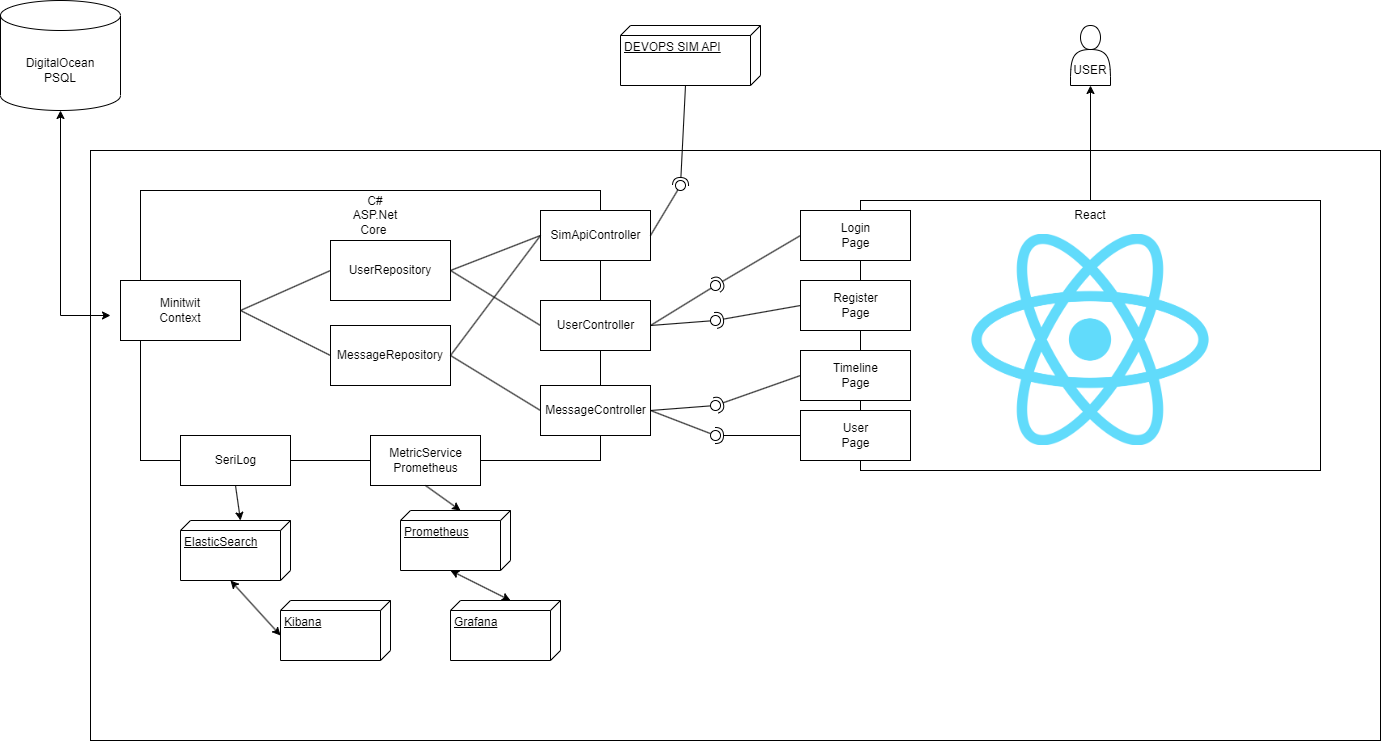
\includegraphics[width=\textwidth]{resources/diagram.png}
    \caption{Deployment diagram over MiniTwit.}
    \label{fig:deploymentDiagram}
\end{figure}

As seen on the diagram there are many Docker containers running different services. All of the containers are configured to be on the same Docker network so they are visible and are able to communicate via the network.
\subsection{Technologies}
The system is developed into the following tech stack (including tools): 
\begin{center}
\begin{tabular}{@{$\bullet$ }ll}
        Backend/API: & C\# ASP.NET core\\
        Frontend: & React (with TypeScript) \\
        Data Abstraction Layer: & Entity Framework Core (EFCore)\\
        Database: & PostgreSQL database \\
        Version Control: & GitHub \\
        Hosting: & DigitalOcean \\
        Containerization: & Docker \\
        Environment Configuration: & Vagrant \\
        Logging: & ElasticSearch, Serilog \& Kibana \\
        Monitoring: & Prometheus \& Grafana \\
        Code Quality: & SonarCloud \& Code Climate\\
        Security: & Snyk \\
\end{tabular}
\end{center}

C\# ASP.NET Core was the choice of API backend as an experiment for the group to use the native ASP.NET Core package for the first time. It has thorough documentation and resources online, making it a solid start when taking the legacy system to the new tech stack. As this is used in workplaces and apps globally, this is also great experience with a professional package that is relevant for developers in the future.

For the frontend, React with TypeScript was used. This is a common way to utilize an ASP.NET Core API, and is hugely common in the professional software engineering world. Several team members had little-to-no experience with React and would have a good learning experience using this in a project of this size. React is for the fifth year in a row the most wanted framework according to stackoverflow\cite{developerSurvey}. It has a continuous large user base, good interoperability and high performance.

EFCore was chosen as the data abstraction layer very early as it is the natural progression when setting up an ASP.NET Core project. It omits much of the database reading and writing and provides a simpler interface for the developers to write business logic and repositories for use with ASP.NET Core.

When transitioning to the new tech stack at the beginning of the project, the database was not changed from SQLite. As performance on the SQLite was decreasing with the amount of users and requests rising the decision was made to change to a PostgreSQL database hosted and managed by Digital Ocean. While migrating to the new database, the group also tested out MySQL on Digital Ocean as well but data transfer was faster on the PostgreSQL database therefore it became the main database and the MySQL one was deleted.

No team members had experience with the use of GitHub in a devops setting, hereunder GitHub actions. The other choice that was considered was Azure DevOps with Azure Pipelines, but a few team members had a lot of professional experience with the entire Azure suite and this made GitHub more attractive as the Version Control and platform for the CI/CD artifacts.
\subsection{Docker}
%relates to "Applied strategy for scaling and load balancing."
Docker has been a key tool for development of the project. It allowed the creation of separate images for different parts of the system, such as frontend, backend, monitoring and logging. Each Docker image encapsulated the dependencies and configurations which ensured reproducibility across environments. Team members could then work in their individual components without worrying about conflicts with other parts of the system. This simplified the development and deployment since it was easier to test each component individually.

Even though Docker helped in terms of deployment and isolation, Docker Swarm was not implemented before deadline. Docker Swarm would have enabled better scalability by deploying clusters of Docker nodes. This would lead to a distributed workload while improving the availability and performance of the system when under heavy load. Each swarm would communicate with each other via the Docker API. Docker swarm makes a system scalable and resilient, ensuring high availability and auto-management. This is in part done by the Docker Swarms built-in automatic load-balancing.

The aforementioned images could have been converted to separate services and then added to the initialized manager node as workers. This ensures that it is possible to scale and replicate the right services. Adding to this, the next step would have been to create back-up managers with replicated workers in case the main manager dies.

\subsection{State of system}

The state of the system have to be reviewed from different perspectives. Code Climate provides the information seen in \autoref{fig:ccstate}.

\begin{figure}[H]
    \centering
    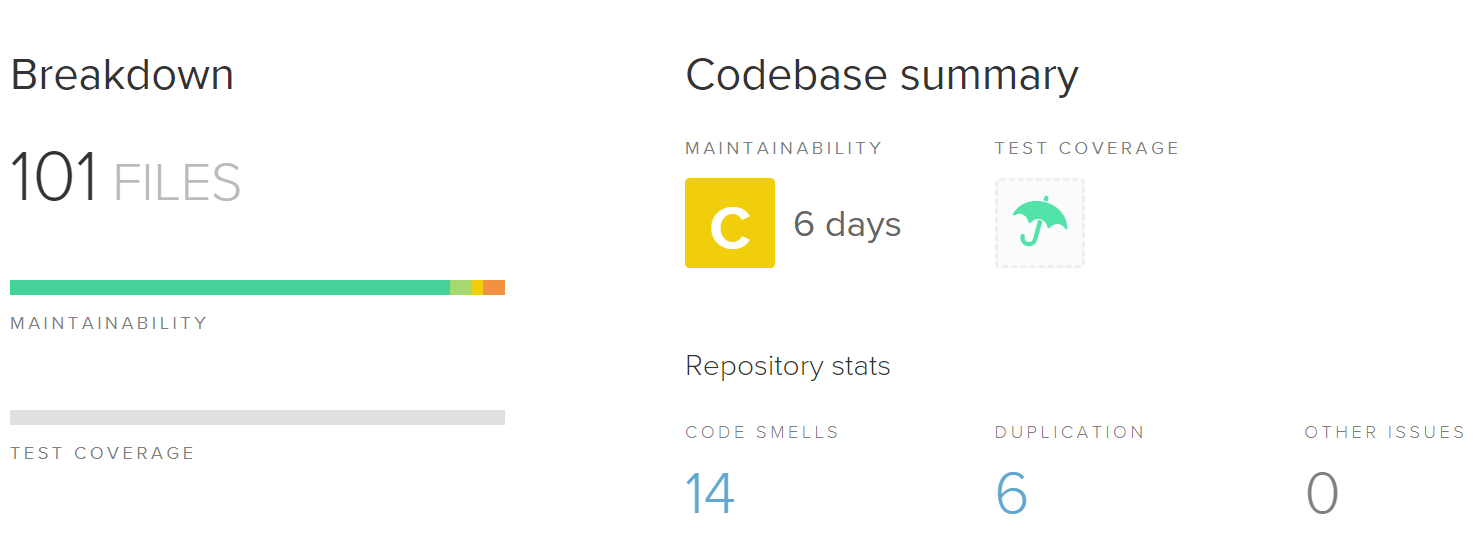
\includegraphics[width=\textwidth]{resources/CCstate.PNG}
    \caption{Codebase summary.}
    \label{fig:ccstate}
\end{figure}

Looking into these issues, many of them concern methods having too many lines of code. System limit is 25, while some happen to contain 40 lines of code. Some of the other smells revolve similar code blocks across different files. Essentially, these issues are categorized as either duplication or complexity.

SonarCloud is another integrated tool with some of the same properties as Code Climate. Taking a look on the summary reveals 36 code smells and a potential critical security issue. A summary of these can be seen below in \autoref{fig:scstate}.

\begin{figure}[H]
    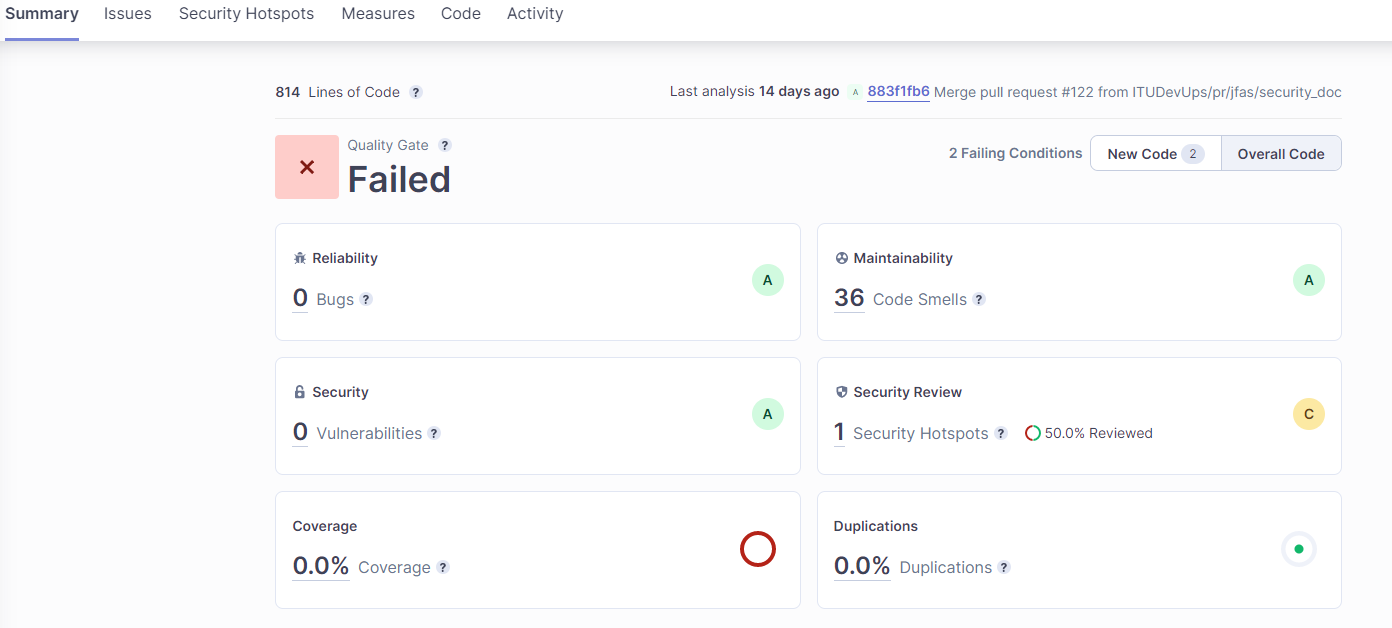
\includegraphics[width=\textwidth]{resources/sonarcloud2.PNG}
    \caption{SonarCloud summary.}
    \label{fig:scstate}
\end{figure}

It provides a deep look into the code smells giving an overview over severity, location, status and if it is assigned to a team member. A view of this can be seen in \autoref{fig:sccodesmells}.

\begin{figure}[H]
    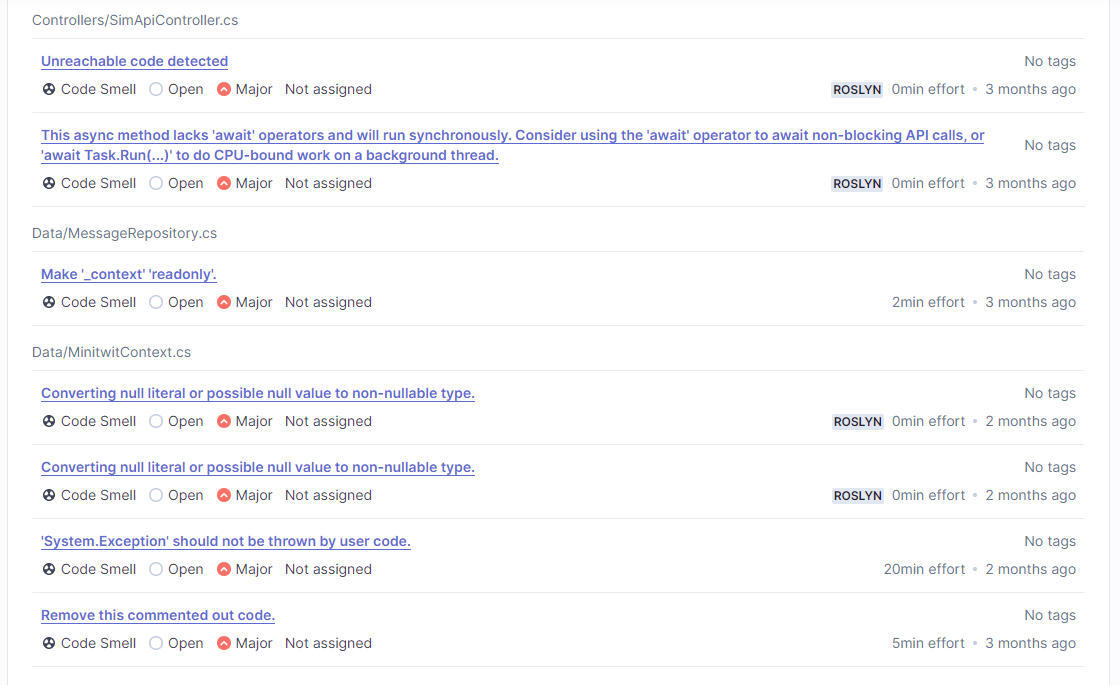
\includegraphics[width=\textwidth]{resources/sonarclouddeep}
    \caption{SonarCloud code smells.}
    \label{fig:sccodesmells}
\end{figure}

Generally, the issues are related to clean code properties such as style, quality, maintainability and design - which in large part is handled by SonarClouds Roslyn\footnote{Roslyn is the codename for the .NET Compiler Platform, used for compiling and understanding C\# code.} integration. The issues in the snippet are the most occurring detections found by SonarCloud at the moment.

The security issue detected in SonarCloud is from the backend-file appsettings.json, where a hardcoded password for digital ocean db-connection is present. The solution would be to tokenize this password as has been done with other repository secrets. SonarCloud does not approve the current state of the program to be deployed to production. These issues are likely from the time before the SonarCloud integration to the CI-pipeline, as a new pull request with these would not have passed the checks in GitHub Actions.

As it is viewable in the two tools, SonarCloud and Code Climate, the overlap of what they have found is not huge. The reports created from both provides a deeper knowledge of MiniTwit and how it can be strengthened in the refactoring phase and mitigated during pull requests. In short, Code Climate excels in eliminating technical debt and SonarCloud excels in ensuring software quality. 
\subsection{License}
The project is distributed with an MIT license.
As a project using MIT license, all software that is not public domain licensed is compatible with the project. Most of the technologies use MIT license themselves, but specifics such as Prometheus and Serilog use Apache 2.0 license, which is also compatible with MIT license.

If using this project, you must also adhere to the licenses of the dependencies in the project , meaning no trademark use of Prometheus and Serilog.
\section{Process' Perspective}
\subsection{Work practice}
The team of \textit{DevUps: DevUps: Delivering Buggy Software Late since 2023} consists of four members, Anders Wagner, Theodor Kier, Mathias Fink and Jens Fastrup. The team has collaborated in-person, through Messenger and GitHub.

The main organization on GitHub, has been integral to organize, maintain and integrate the code of the project. This includes creating issues, handle releases, tracking progress, and verifying new work with static analysis.

\subsubsection{Branching strategy}
With the MiniTwit repository on GitHub, it has been possible to adhere to a version control, where proper branching has been an essential part of the development process. At the early beginning of the development a guide on how to contribute to the project was created. This guide can be found on the GitHub repository as \textit{contributing.md}.\\

The guide describes how the GitFlow workflow\cite{gitflow} have been used for development. The \textit{main} branch is the top branch from which releases are created from. The only branch that can push to main is the development branch \textit{dev}. This branch has at every new release the same state as \textit{main}, but it is this branch that team members create new branches from and push work to. Contributing work has to come from a branch that is prefixed with either a \textit{issue number} or as \textit{hotfix}. The branch name describes what it aims to solve. This ensures that team members can easily see what issue a branch is related to.

The issues were posted in \textit{GitHub Project} which resembles a kanban board. This board was used to give a graphical view of the state of issues. Each issue could be marked as either \textit{New, In progress, In review or Done}. It was also possible to see which team member was assigned to which issue. 

Pull requests are linked to issues in the backlog. Likewise, in the process of reviewing pull requests, there is a workflow with several static analysis tools that are implemented with GitHub Actions to guarantee a certain standard of delivered work.

In order to build a proper project, convenience for discovering errors, fixing them and reviewing work is essential. In this aspect, the team has had the mindset of making commits often, in the sense where it reflects a precise, substantial change. Optimally, the team creates a release every week, that reflects a set of fixes, changes and additions. This has not been the case every week, as work in some periods has been solved in bulk, or have had prior work pending. 

\subsection{CI\textbackslash{}CD}

\subsubsection{Continuousdeployment.yml}
The deployment workflow is activated once there is a push to the main branch, which happens after a successful merge. First it logs into Dockerhub which contains the images, then it builds and pushes the newest images from the main branch. After this it SSHs into the Digital Ocean droplet and runs the deploy.sh script which pulls the newest docker images and runs the docker containers


\subsubsection{Other workflows}
Three tools that are present in the CI-workflow on top of the continuous deployment Github Action are:
\begin{itemize}
    \item .Net Test-action, run C\# tests on the backend before deployment.
    \item Snyk-Security, catch vulnerabilities in the language specific domain, before they reach production.
    \item SonarCloud, to ensure code quality and no detectable vulnerabilities.
\end{itemize}

These are run on pull requests going to \textit{main} and \textit{dev} to help ensure the quality of code are up to the standard set by the specific workflows.
\subsection{Monitoring}

Monitoring of the system was done with Grafana and Prometheus.\\
Prometheus is a "Open source systems monitoring and alarms toolkit" that was used to collect and store metrics in relation to the systems performance. \\
Grafana is a open-source web application used for analytics and visualisation. These two solutions were used together in this project to gather data and visualise it to analyze the platform in real-time.

Prometheus and Grafana was setup in each their Docker image and connected to the same Docker network as the images for backend and frontend. The backend was instructed to use Prometheus by setting the port for the backend (3005) as the metrics server of the application. 

A settings file for Prometheus was created that contained various configurations. These included the scraping interval, what port Prometheus should be available on (9090) and what was the target for scraping data (minitwitbackend:3005).

In Grafana's settings a new data source was added for Prometheus and the port it was running on. This data source was used for every panel created in the Dashboard. Each panel had a query in it that decided what data was shown in the panel. The dashboard consisted of five panels: CPU usage, Number of threads, failed requests, successful request, backend memory usage.

Real-time CPU monitors usage to identify if there are any performance bottlenecks or needs for resource optimization.

The active number of threads can be used for assessing system concurrency and identify if there are any potential issues. The same goes for the backend memory usage which can detect if there are any memory leaks or optimizations needed.\\
Failed  request can be used to see if there are service errors in the backend, while successful requests can provide insights into the systems stability and efficiency. It is also an indication of how active users are.

\subsection{Logging}
For implementing the logging of the system, the ELK stack was added. The stack consists of Elasticsearch and logstash Kibana. To get an optimal experience of the ELK stack serilog was implemented in the C\# backend to be able to custom log the API endpoints, however this aspect was not fully utilized.
\subsection{Security}
\subsubsection{Automated Risk Assessment}
A number of vulnerabilities present in MiniTwit was exposed by OWASP ZAP scanning tool. This tool is useful for penetration testing a hosted web-application for vulnerabilities and other security concerns. This practice should be repeated as the application expands with more surfaces to attack and manipulate. This tool is also complementary to some of the static analysis tools implemented in GitHub Actions. No critical issues were detected, only medium to low alerts.

During maintenance, the team tried to change the \textit{X-Content-Type-Options} to \textit{nosniff}. It instructs the browser to always use the MIME-type that is declared in the Content-Type header rather than trying to determine the MIME-type based on the files content. For some reason, the web-application response header did not change, even when the appropriate measures in the middleware were taken. 
    
\subsubsection{Mitigation of Vulnerabilities}
Several steps were taken to ensure the security of MiniTwit. Mainly Snyk, which is a security tool in GitHub performing static analysis in regards to corrupted dependencies. Snyk can be added as a GitHub Action, to secure pull requests. Having a mix of security tools and practices reduce the likelihood of a security breach in terms of confidentiality, integrity and availability. 

\section{Lessons Learned Perspective}
\subsection{Evolution \& refactoring}

During the start of the refactoring is was primarily focused on creating the new frontend and make the backend able to retrieve the messages from the database for the frontend, and make the backend work for the simulator. This was due to a large workload and time constraints, so tests and the database was not refactored initially.

This prioritization was done based on what is more tangible. Creating the new frontend and ensuring the backend worked with the simulator were considered the "bare minimum" for the functionality and made it seem like an updated system for the users point of view. Other areas would have to be done at a later stage.
Refactoring the whole codebase at once can be overwhelming and time-consuming. By doing an incremental approach after creating something that looked new and worked, it was possible to improve areas one at a time without disrupting the system's functionality.

\subsubsection{Testing}
Some issues related to this approach was also that some areas was not prioritized or simply not recognised at first. The date for messages was wrong for a while because it was not noticed.
Manual testing was prioritized instead of refactoring the tests from the legacy codebase. When a new feature was developed the frontend was tested by group members simply using the new parts and look at them in a browser to check for errors. For the backend, a .NET testing-action was setup in GitHub Actions. This action would ensure that future tests related to the backend would be evaluated before being merged to \textbf{dev}. This aims to preserve the behavior of test-covered code.\newline If the project had refactored tests before the continuous development of new features fewer issues might have occurred during the development.

\subsubsection{Database}
The database migration was done a few weeks after the start of the simulator. The amount of entities (user, messages etc.) was continually increasing. The time needed for the database migration would have been less if done earlier in development. 

\subsection{Operation \& Maintenance}
\subsubsection{CORS}
During the early refactoring of the codebase there were issues related to retrieving data to the frontend from the API. This issue was caused by cross-origin resource sharing (CORS). CORS is used set as an HTTP header that instructs the server to state which domains other than its own, that it allows loading resources from. Due to the groups limited experience with the technologies the team had to search documentation on how to implement CORS in both the frontend and backend.

In the frontend the solution was to set the \verb|mode: cors| for the fetch. In the backend it was to make the builder add CORS to its services. After the app-object was created, it was instructed with the following arguments \verb|app.UseCors(builder => builder.AllowAnyOrigin()|\\
\verb|.AllowAnyHeader().AllowAnyMethod())|. These can be seen implemented in commit \textit{272da82e50732c8f9b4a458598456b4d27e23350} and \\\textit{584bee004b75397d181383a66b77dd3985bad23f}.

This issue was difficult to find as there was a difference in how CORS worked depending on how you tested it locally or if it was deployed on the DigitalOcean server. And even if you tested it locally with or without the docker containers.

\subsubsection{Logging early}
After converting the legacy code to the new tech stack, a lot of issues came up when the simulator was posting tweets and users.\\
This was related to an issue with asynchronous code and was very difficult to track down until logging was implemented.\\
The fix was not trying to post everything asynchronously, but rather to just save the state of the database asynchronously.\\
This was fixed in commit \textit{0c3a1f32b398138c9c531495643ae0d046e42fc1};

Having logging earlier would have helped in solving this issue, so the issue persisted for several weeks and contributed to many features getting delayed several weeks.

\subsubsection{Wrong date formatting}

When refactoring from the python application to the project tech stack, there were issues finding out how to handle date times.\\

The date times were saved as natural numbers in python and it was not described if it was the amount of ticks, seconds, minutes or what it was. Later in the project it was found out that it was the amount of seconds since 1970. When implementing the date time data in the C\# implementation, there was some miscommunication about the format of the data and this resulting in the format of dates being saved as a casted int of ticks, making the dates range from 1970 to 2034 when displayed in the frontend. \\

The issue was not fixed and all the old wrong data was not migrated. The solution to fix the old data was to reset them (as it was mostly just simulator data) if they were outside a range of 1970 and the current date, migrating the data would be done in batches to omit straining the system too much during load hours.

\subsubsection{Memory leaks at frontend}

During development, memory leaks were introduced in the frontend code. One type of leaks was due to fetch-methods missing a necessary dependency in their calls. This resulted in the methods being invoked repeatedly, leading to resources constantly being fetched thus increasing the transfer size. This made the site either very slow or unusable in periods.

Another memory leak was due to the frontend trying to fetch all messages at once. In the early stages of development this was not an issue, but as the simulator generated an increasing number of messages in the database, the workload of fetching these messages increased. A few weeks into the development, this workload became so big it caused a significant delay in loading the messages at the frontend. Additionally, if the frontend was tested locally, the high workload could overload the node causing it to crash.

This proves the importance of an early analysis of tasks that may have a significant workload for the server as the amount of data increases. If this was done the performance of the system would have been increased and ensured that it could handle higher loads.
\newpage
\section{Conclusion}
The group has during the course taken a legacy MiniTwit python application and have developed it to a new tech stack using DevOps praticies and DevOps techniques such as logging, monitoring and automatic CI/CD \\

Throughout the project, the advantages of adopting DevOps principles and implementing artifacts became increasingly apparent. Not only were mistakes detected and resolved more efficiently during development, but deployments and quality control processes were also automated, accelerated, and more reliable. \\

The project served as an invaluable learning platform, allowing the team to apply DevOps techniques rather than simply studying them theoretically. This hands-on experience also exposed them to the challenges and complexities of configuring a system of this size. By providing a safe environment for DevOps, the project encouraged experimentation with various tools and technologies, even those unfamiliar to the team members. \\

As a result, the developers acquired firsthand insights into the benefits of DevOps, which they will carry forward into their future hobby projects and professional software careers. With this knowledge, they are better equipped to drive efficiency, collaboration, and robustness in their future developments. The project not only exemplified the power of DevOps but also empowered the team to embrace DevOps in their ongoing software development journey.

\newpage
\printbibliography

\newpage
\appendix

\section{Appendix}
\subsection*{ZAP scanning report}
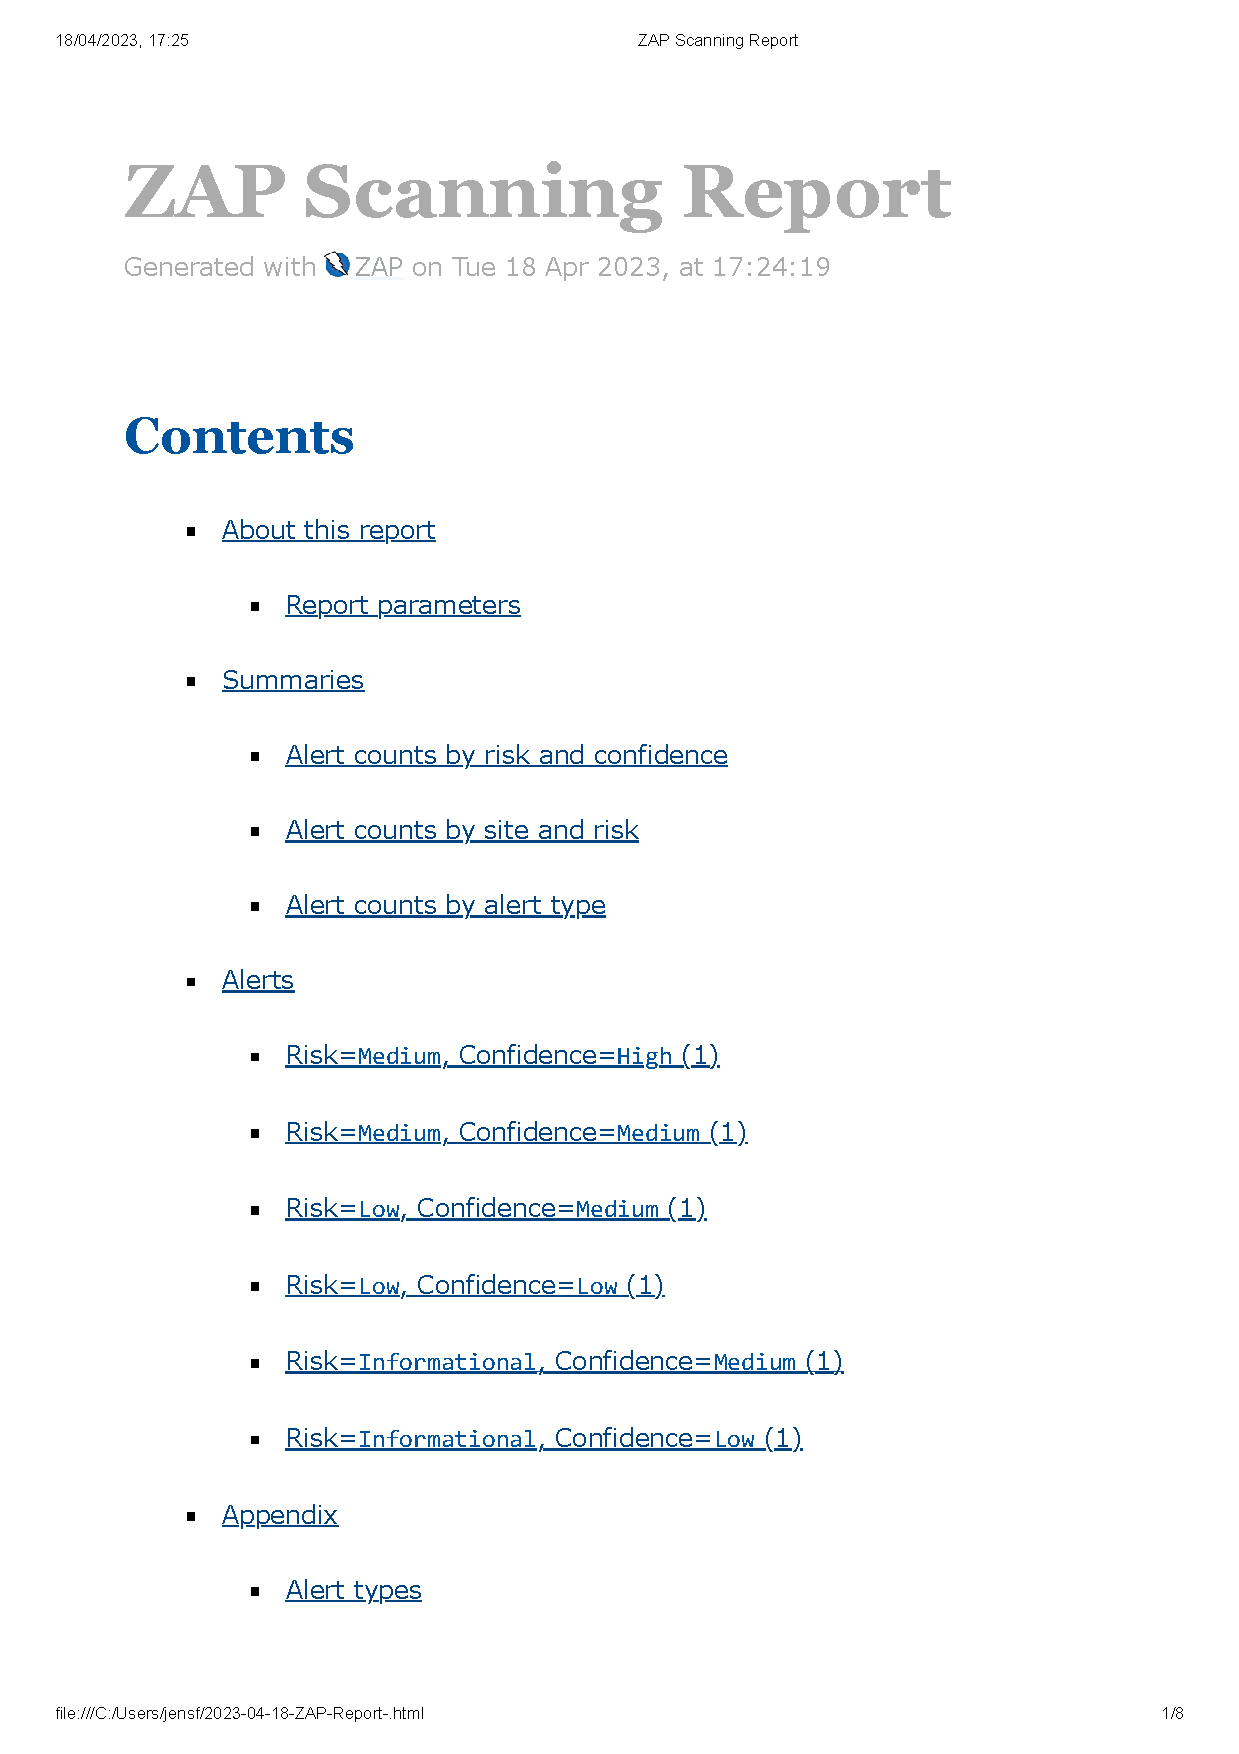
\includepdf[pages={-}, width=\textwidth]{resources/zap.pdf}


\end{document}
